\documentclass{article}
\usepackage{color}
\usepackage{placeins}
\usepackage{listings}
\usepackage{graphicx}
\usepackage{xcolor}
\usepackage{amsmath}
\usepackage{subcaption}
\usepackage{cleveref}
\usepackage{geometry}[margins=1in]
\setlength{\parskip}{4pt plus 2pt}
\setlength{\parindent}{0pt}
%\pagecolor[rgb]{0,0,0} %black
%\color[rgb]{1,1,1} %grey
\lstset{language=C++,
keywordstyle=\color{blue},
stringstyle=\color{red},
commentstyle=\color{green},
morecomment=[l][\color{magenta}]{\#},
breaklines=true,
breakatwhitespace=true,
numbers=left
}
\title{Assignment \#4}
\author{Asbjørn Bonefeld Preuss,\\ Daniel Lomholt Christensen,\\ Elie Cueto}
\date{March 2024}

\renewcommand{\thesection}{Task \#\arabic{section}}
\renewcommand{\thesubsection}{\arabic{section}.\arabic{subsection}}
\begin{document}
\maketitle
\section{Parallelising the code}\label{sec:taskone}
In order to parallelise the code, we first profiled the sequential code. This result can be seen in appendix \ref{sec:Profiling}. The profiling showed that our initial effort should be concentrated around the propagator function, and then next address the fourier transformation, and finally the inverse fourier transformation.

The propagator function was parallelised by first beginning a parallel block on line 178, as soon as all the important declarations and initialisations are done. This block ends just before the function prints out the debugging information and ends the time taking, at line 278. 

Inside the parallel block, all for loops are given an omp for directive, thus spreading the loop iterations over the threads. Omp single directives are used when only one thread must execute the code. This is all that was used to parallelise the propagator function.

Next, the fast fourier transformation(lines 104-129) was parallelised. Since the fft is a recursive function, the most important part to parallelise is the calling of the function itself. We do not want to parallelise the for loops, because each time the function is called a new, the threads must be spun up anew, as they cannot be used for calling the function again.

The fft calls inside the fft function are therefore just given to a thread, and then the computer is asked to wait until the tasks finish.

Finally the inverse fast fourier transform(lines 132-152) is parallelised. The ifft is run in parallel, with the two loops getting the omp for directive, and the fft call given on only a single thread. The second loop is split, into a vectorisable part and non-vectorisable part, and given the appropriate directives to compile it correctly.

The overall strategy is therefore to parallelise what can be parallelised, if there is any gain to be made from the parallelisation.

We tested that the checksum is the same, 23.2912755963295 for the vectorised, and 23.2912755963295 for the sequential code, run with $n_{freq}=2^{16}$. 

\section{Scaling}
\subsection{Strong scaling}
In order to investigate the strong scaling of the problem, three versions of the parallelised code were compiled. The first having only gotten added pragmas in the propagator function, the second having been optimised in the FFT-function, and the last having some parallelisation added to the IFFT-function as described in the previous section.

Each of these programs were then asked to solve the inverse problem with \(2^{20}\) frequencies in the spectrum. Afterwards, we fitted Amdahl's law to the data points and got that the serial part of the code was 7\% in v1, 5\% in v2, but in v3, where we tried to parallelise the inverse fourier transform, the added overheads made the code slower, with 6\% serial source code.
For completeness, this corresponds to 93\%, 95\%, and 94\% parallel code for the first, second, and third version respectively.
\begin{figure}
    \centering
    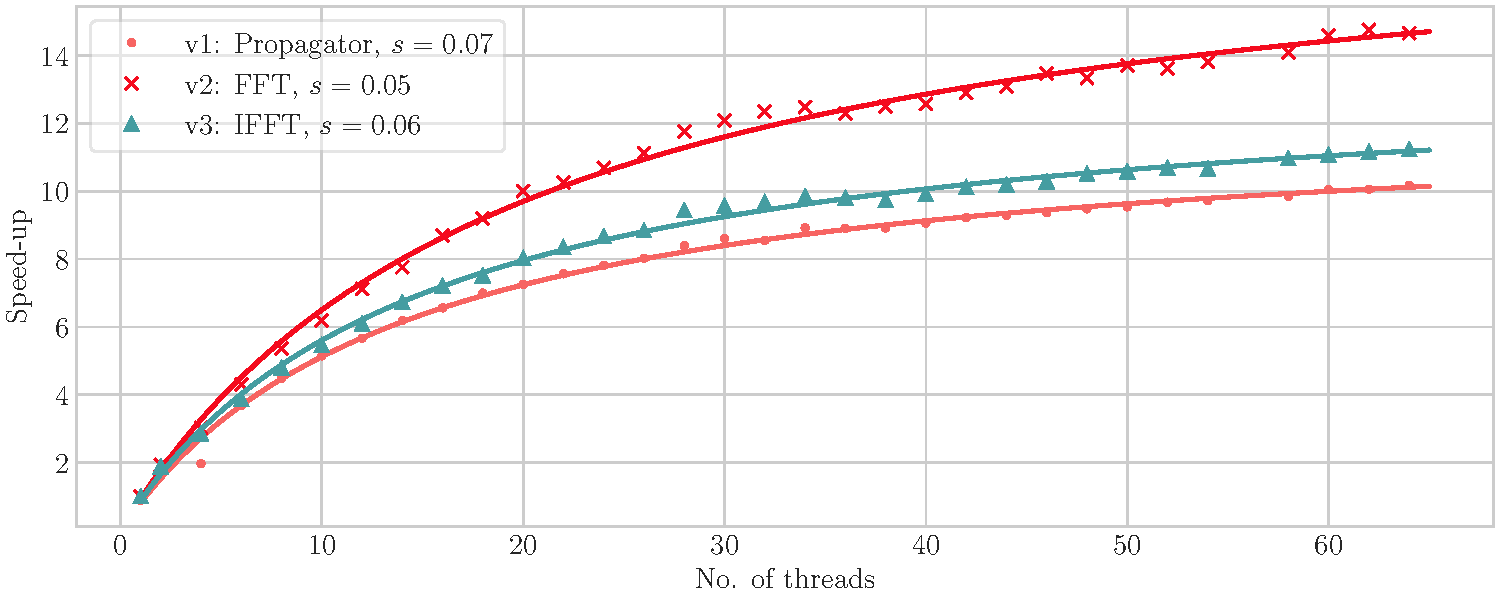
\includegraphics[width=\textwidth]{./figures/amdahl.pdf}
    \caption{The strong scaling of the three different versions of the program.}
    \label{fig:amdahl}
\end{figure}

\subsection{Weak scaling}
For weak scaling, we mulitplied the amount of frequencies in the spectrum by the amount of available cores. Which, if all of the code scaled linearly would give us a simple linear relationship in time and a constant speed-up. However, the Fourier Transform is using a divide and conquer approach, resulting in $\mathcal{O}(N\log N$ operations, for a problem of size $N$. This means that the rest of the code executes in a constant amount of time, but the transforms keep on taking longer and longer as seen in \cref{fig:fft_scaling}. To take this into account, we scaled the speed-up with the scale of FLOPS,
\begin{align}
    S &= \frac{t_{seq}}{t_\text{no fft} + \log(N) \cdot t_\text{fft}} \cdot N.
\end{align}
This relationship is plotted in \cref{fig:weak}.
%In the report it is expected that you interpret and discuss your scaling results. You should interpret them considering the code, the workload, and in the context of the shared memory architecture of ERDA.
\begin{figure}
    \centering
    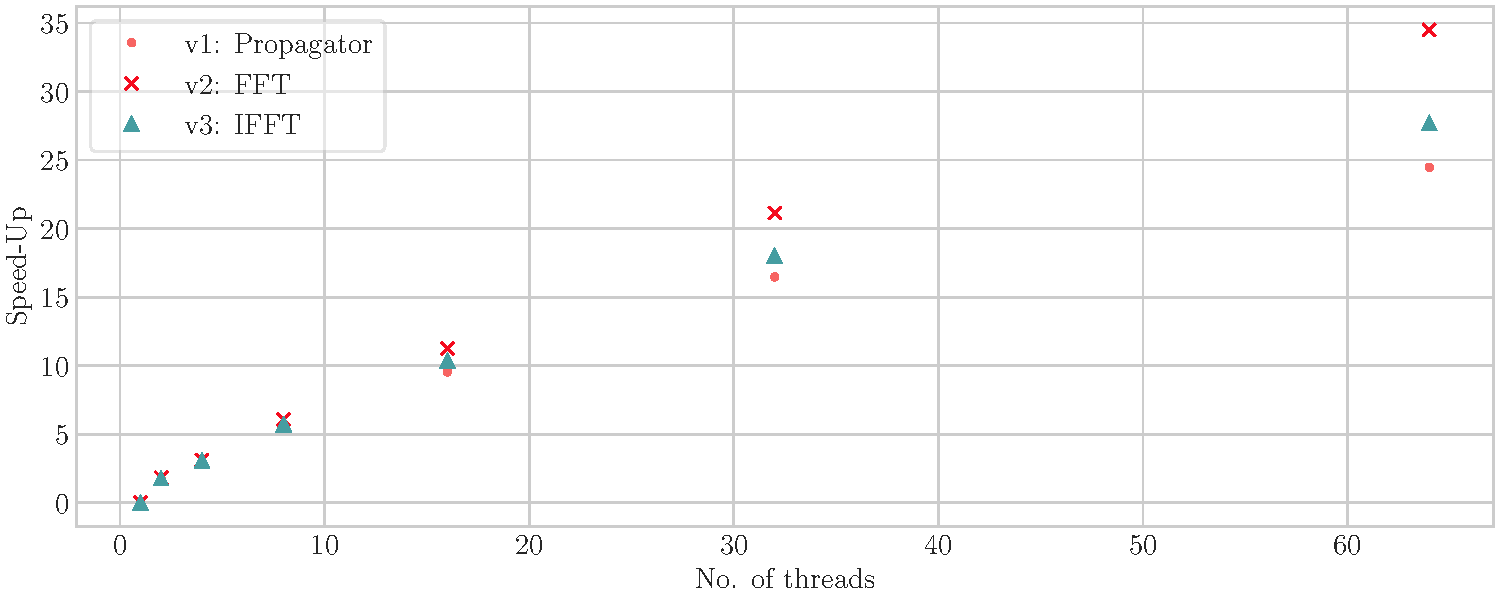
\includegraphics[width=\textwidth]{./figures/weak_scaling_corrected.pdf}
    \caption{Weak scaling of the code. The Speed-Up is corrected for the extra FLOPS of the larger data_sets}
    \label{fig:weak}
\end{figure}

\begin{figure}
    \centering
    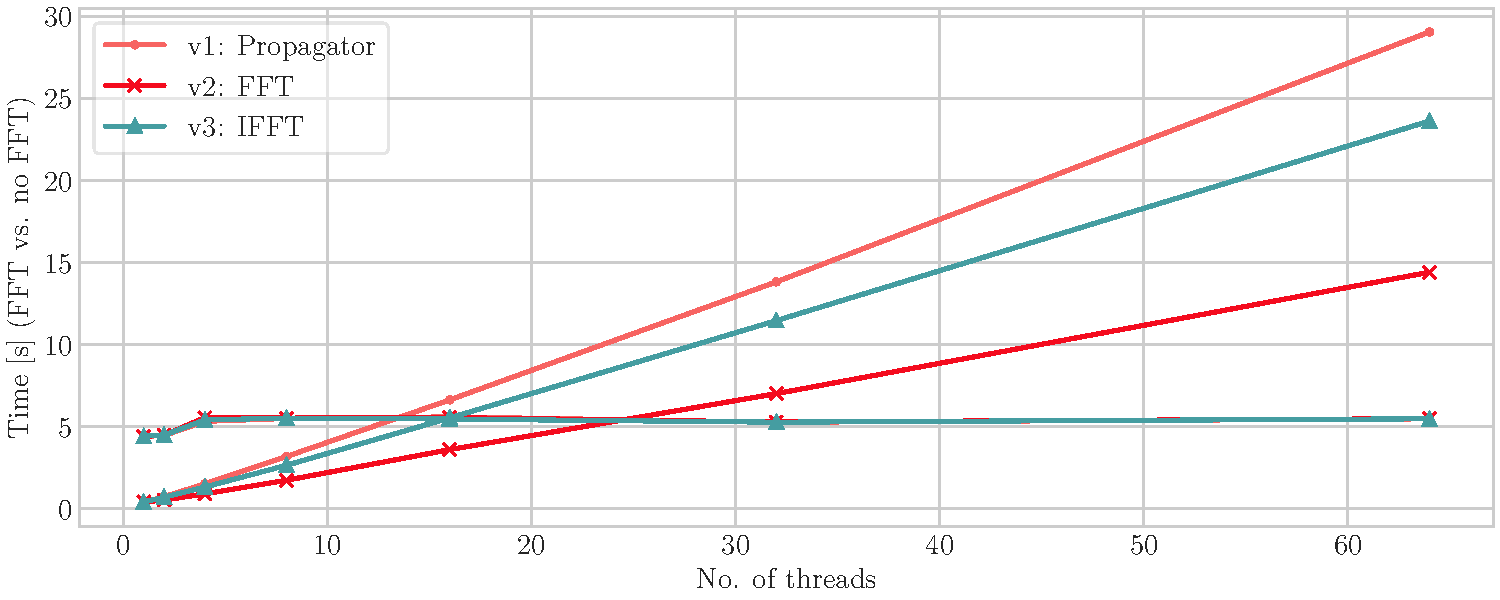
\includegraphics[width=\textwidth]{./figures/FFT_scaling.pdf}
    \caption{The scaling of the part of the code involving Fourier transforms, and the rest of the code. The former clearly rising with the scaling of the number of threads/problem size, and the latter remaining constant.}
    \label{fig:fft_scaling}
\end{figure}

\appendix
\newpage
\section{Profiling}
\label{sec:Profiling}
\begin{figure}[h]
    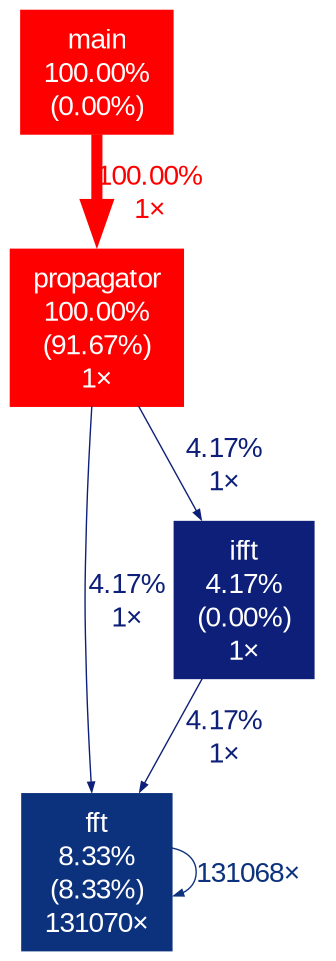
\includegraphics[height=0.6\textheight]{figures/gprof_seq.png}
    \centering
    \caption*{Profiling of the sequential program.}
\end{figure}
\FloatBarrier
\section{Source Code}
\label{sec:source}
\lstinputlisting[language=c++]{../Code/seismogram_omp.cpp}

\end{document}
